\documentclass{beamer}
 
\usetheme{Madrid}
\makeatletter
\newcommand{\rmnum}[1]{\romannumeral #1}
\newcommand{\Rmnum}[1]{\expandafter\@slowromancap\romannumeral #1@}
\makeatother
 
%Information to be included in the title page:
\title[DL for hurricane track forecast ] %optional
{Fused Deep Learning For Hurricane Track Forecast From Reanalysis Data}


\author{Mo YANG}


\institute[u-psud] % Your institution as it will appear on the bottom of every slide, may be shorthand to save space
{
	Supervisor: \\ % Your institution for the title page
	\medskip
	Claire Monteleoni
	\\
	Guillaume Charpiat 
	\\
	Sophie Giffard-Roisin
}
\date{\today} % Date, can be changed to a custom date
 
 
 
\begin{document}

\begin{frame}
\titlepage % Print the title page as the first slide
\end{frame}


%----------------------------------------------------------------------------------------
%	PRESENTATION SLIDES
%----------------------------------------------------------------------------------------

%------------------------------------------------
\section{Background} % Sections can be created in order to organize your presentation into discrete blocks, all sections and subsections are automatically printed in the table of contents as an overview of the talk
%------------------------------------------------
\subsection{Hurricane Track Forecast}

\begin{frame}
\frametitle{Outline} % Table of contents slide, comment this block out to remove it
\tableofcontents[currentsection] % Throughout your presentation, if you choose to use \section{} and \subsection{} commands, these will automatically be printed on this slide as an overview of your presentation
\end{frame}


\begin{frame}
\frametitle{Hurricane}
\begin{itemize}
\item Cyclones, hurricanes or typhoons: words for the same phenomena
\item Cost tremendous damage and death each year
\item Can be very unpredictable.
\item \textbf{Tracks} and \textbf{Intensity} : Two main goals of the forecast
\end{itemize}
\end{frame}

\begin{frame}
\frametitle{Hurricane}
\begin{itemize}
	\item The evolution and path of the hurricane Katrina (2005) \\
\end{itemize}
\begin{figure}
	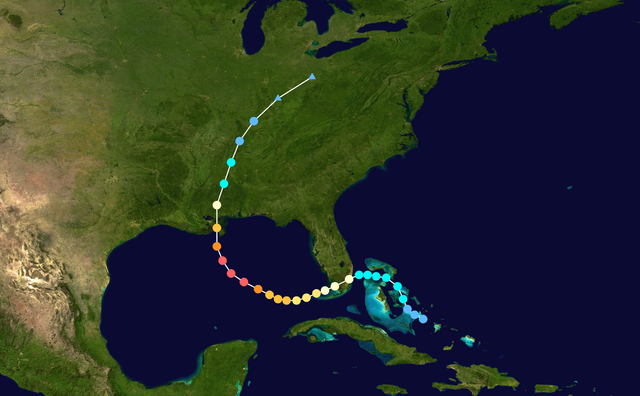
\includegraphics[width=0.6\linewidth, height=0.6\textheight]{figs/Katrina.png}
	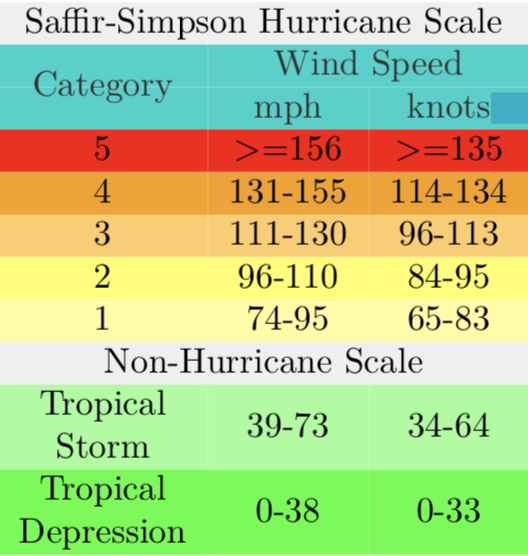
\includegraphics[width=0.3\linewidth, height=0.4\textheight]{figs/saffir-simpson.png}
\end{figure}
\end{frame}



\subsection{Hurricane Track Forecasting Models for Meteorologists }



\begin{frame}
\frametitle{Guidance Models}
\begin{itemize}
	\item Statistical models: do not consider physics, generate forecast in seconds. e.g. Best Track Decay (BCD5)
	\item Dynamic models: solve the physical equations governing the motions in the atmosphere, more accurate but computationally demanding. 
	\item Official NHC forecast (OFCL) :  consensus models which are created by combining the forecasts from a collection of other models.
\end{itemize}
\end{frame}
 

 
\section{Preliminaries}
\begin{frame}
\frametitle{Outline} % Table of contents slide, comment this block out to remove it
\tableofcontents[currentsection] % Throughout your presentation, if you choose to use \section{} and \subsection{} commands, these will automatically be printed on this slide as an overview of your presentation
\end{frame}

\subsection{Problem Setting}
\begin{frame}
\frametitle{Problem Setting}
\begin{itemize}
	\item Goal: estimating the 24h-forecast trajectory of all tropical storms.  \\
\end{itemize}
\begin{figure}
	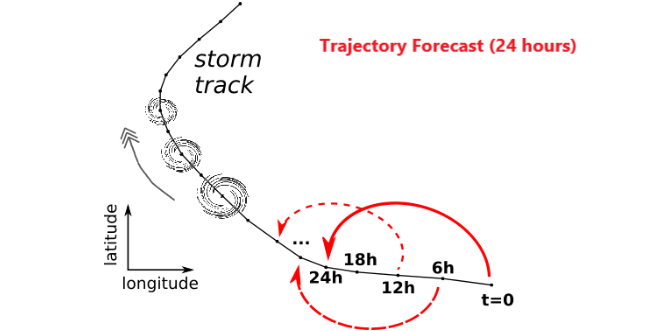
\includegraphics[width=0.8\linewidth]{figs/storm_shema.png}
\end{figure}
\end{frame}

\subsection{Previous Works}

\begin{frame}
\frametitle{Previous Works}
\begin{itemize}
\item A large family of previous methods used spatio-temporal features
\begin{itemize}
	\item Two-stream Convolutional Network
	\cite{simonyan2014two}
	\item Convolutional LSTM \cite{xingjian2015convolutional}
	\item Temporal Convolutional Networks \cite{lea2016temporal}
\end{itemize}
\item Only two preliminary studies have tackled the hurricane forecast tracking using machine learning
\begin{itemize}
	\item Use random forests on local reanalysis histograms \cite{liberge2011prevision}
	\item Train a sparse recurrent neural network from trajectory data \cite{moradi2016sparse}
\end{itemize}

\end{itemize}
\end{frame}
 
 \section{Method}
 \begin{frame}
 \frametitle{Outline} % Table of contents slide, comment this block out to remove it
 \tableofcontents[currentsection] % Throughout your presentation, if you choose to use \section{} and \subsection{} commands, these will automatically be printed on this slide as an overview of your presentation
\end{frame}
\subsection{Data Description}



\begin{frame}
\frametitle{Data sources}
\begin{itemize}
	\item  \textbf{Storm track data}: composed of tropical/extra-tropical storm tracks since 1979 extracted from the NOAA database IBTrACS. \\
	\begin{figure}
		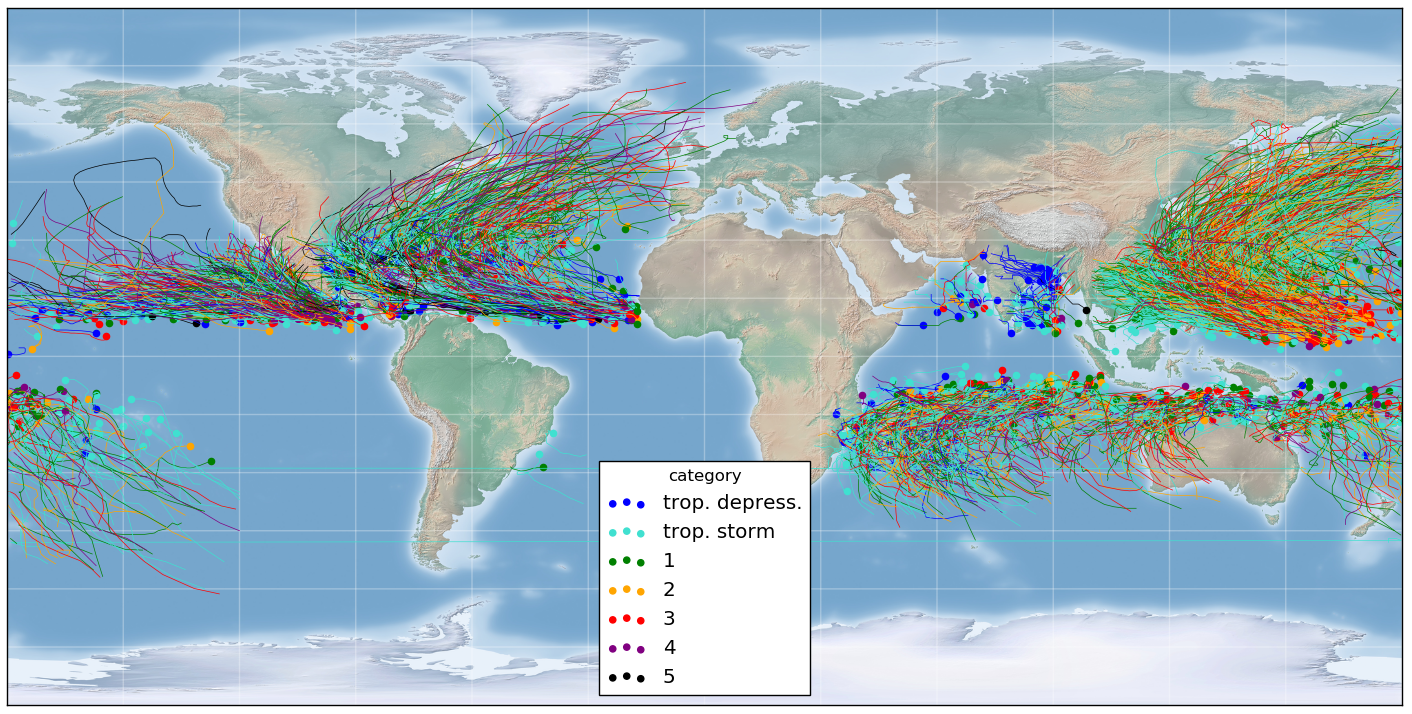
\includegraphics[width=0.7\linewidth, height=0.5\textheight]{figs/all_storms.png}
		\label{fig: storm_tracks}
		\caption{Database: tropical/extra-tropical storm tracks since 1979. Dots = initial position, colors = maximal storm strength according to the Saffir-Simpson scale.}
	\end{figure}
\end{itemize}
\end{frame}

\begin{frame}
\frametitle{Data sources}
\begin{itemize}
	\item \textbf{Reanalysis:} the latest global atmospheric reanalysis ERA-Interim produced by The European Centre for Medium-Range Weather Forecasts (ECMWF). 
	\begin{itemize}
		\item global atmospheric fields : u-wind, v-wind, pressure, temperature, humidity, vorticity ... every 6 hours
		\item spectral resolution: about 80km on 60 vertical levels from the surface up to 0.1 hPa
	\end{itemize}
	\begin{figure}
		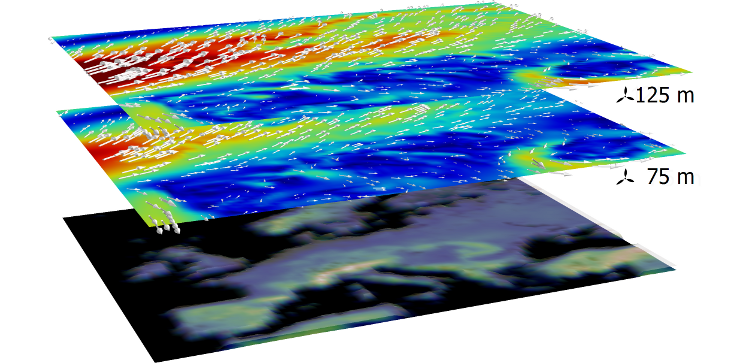
\includegraphics[width=0.7\linewidth, height=0.4\textheight]{figs/Reanalysis-Data-Wind-Speed.png}
		\caption{Reanalysis wind fields (Source: from website)}
	\end{figure}
\end{itemize}
\end{frame}


\begin{frame}
\frametitle{Input features}
\begin{itemize}
	\item \textbf{The wind fields.} u-wind and v-wind fields on a 25x25 degree grid centered on the current storm location, at three atmospheric pressure levels (700 hPa, 500 hPa, and 225 hPa),  from consecutive previous - current time point \textbf{(3D tensor)}
	\item \textbf{The pressure fields.} geopotential height fields on a 25x25 degree grid centered on the current storm location, at three atmospheric pressure levels (700 hPa, 500 hPa, and 225 hPa), from consecutive previous - current time point \textbf{(3D tensor)}
	
\end{itemize}
\end{frame}

\begin{frame}
\frametitle{Input features}
\begin{itemize}
\item \textbf{Storm track in history.}  The past 6-hourly displacement in lat. and lon. \textbf{(1D tensor)} 
\item \textbf{Other hand-crafted features:} current lat. and lon.,  windspeed, Jday predictor(Gaussian function of "Julian day of storm init - peak day of the hurricane season"\cite{demaria2005further}), and current distance to land.  \textbf{(1D tensor)} 

\end{itemize}
\end{frame}


\subsection{The proposed method}
\begin{frame}
\frametitle{Overview of the proposed method}
\begin{itemize}
	\item  Three-stream fusion network \\
\end{itemize}
\begin{figure}
	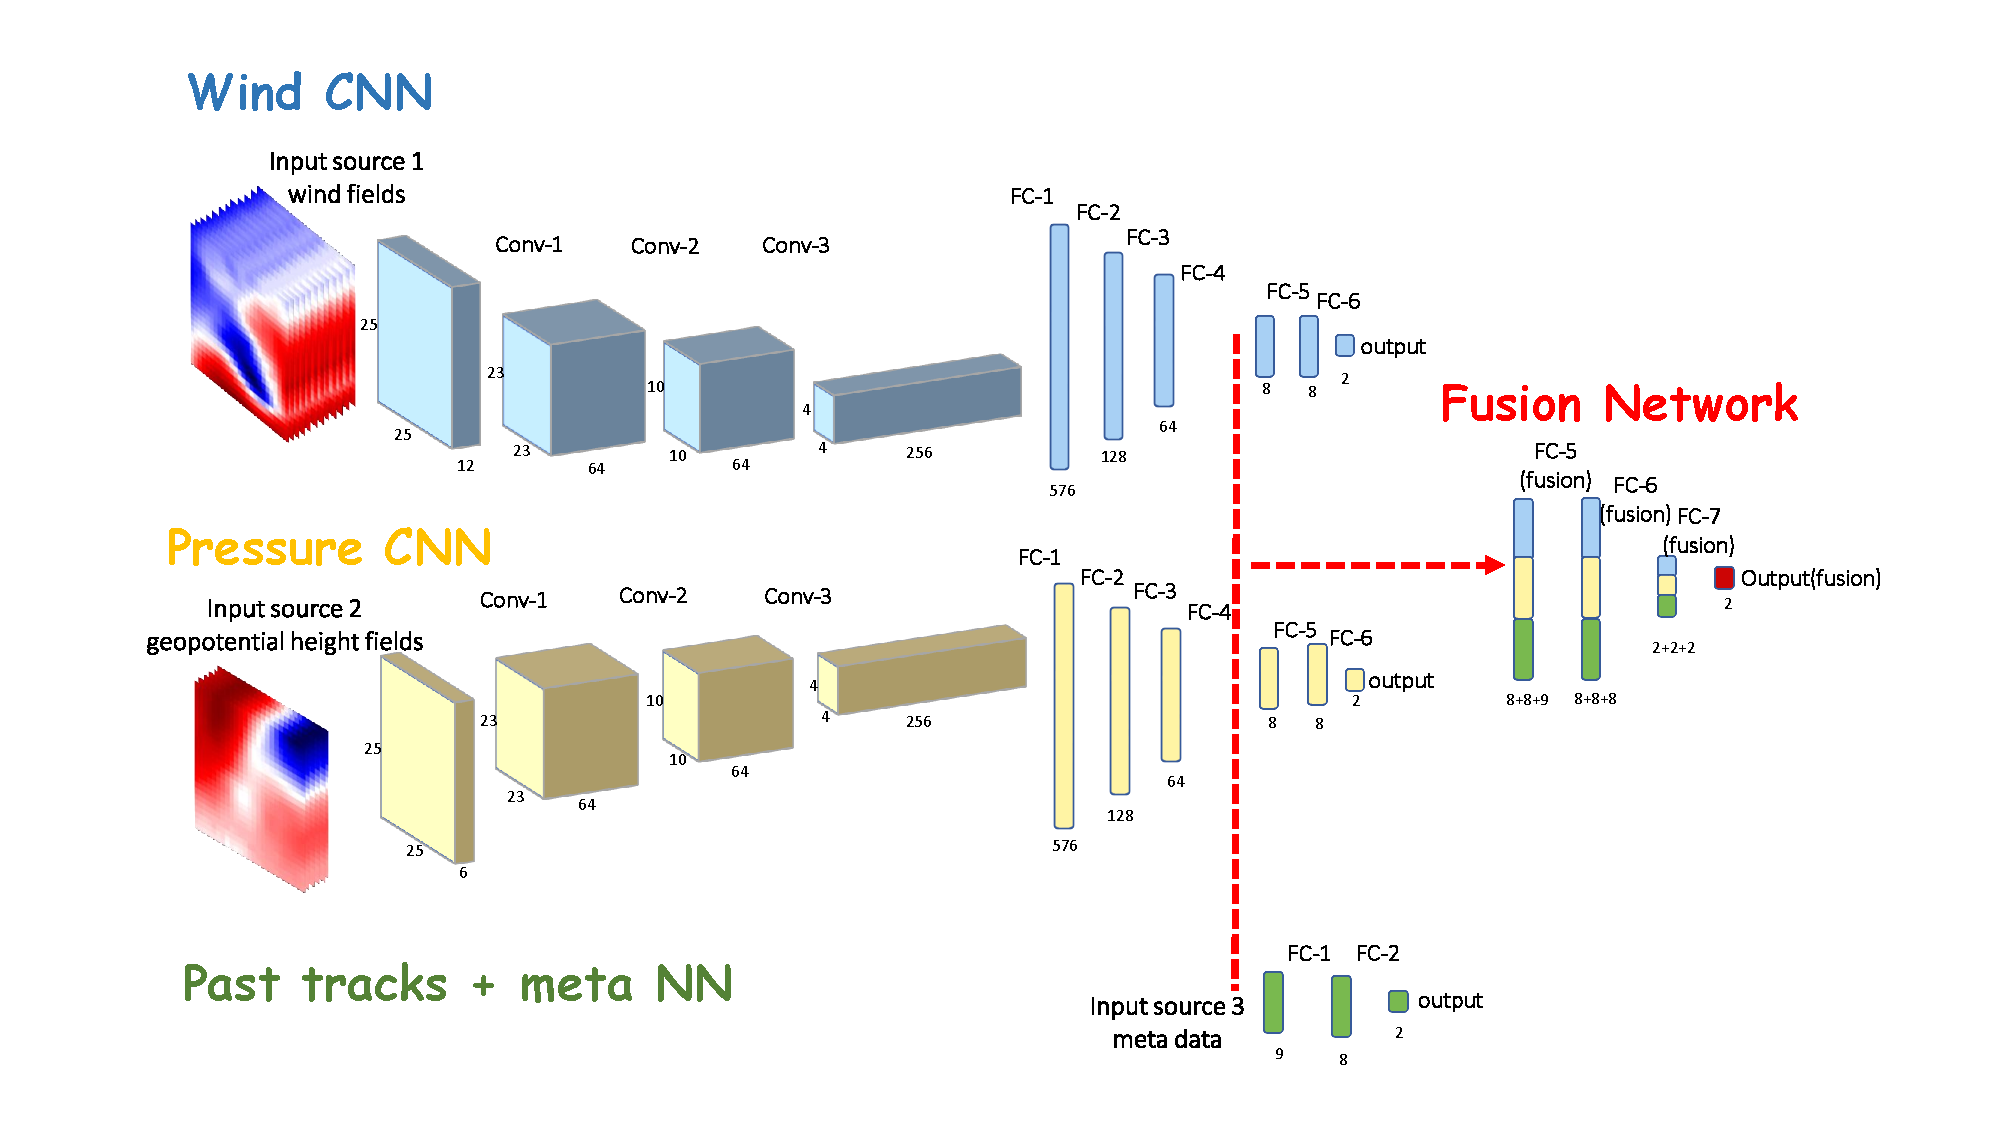
\includegraphics[width=1.0\linewidth]{figs/fusion_network.pdf}
\end{figure}
\end{frame}


\begin{frame}
\frametitle{Train Stream Networks}
\begin{itemize}
	\item  Stage \Rmnum{1}: Train stream networks \\
	\begin{itemize}
		\item Wind CNN
		\begin{itemize}
			\item pretty standard (popular) CNN architecture, like VGG Net \cite{simonyan2014very}
			\item trying from shallow to deep
		\end{itemize}
	\end{itemize}
\end{itemize}
\begin{figure}
	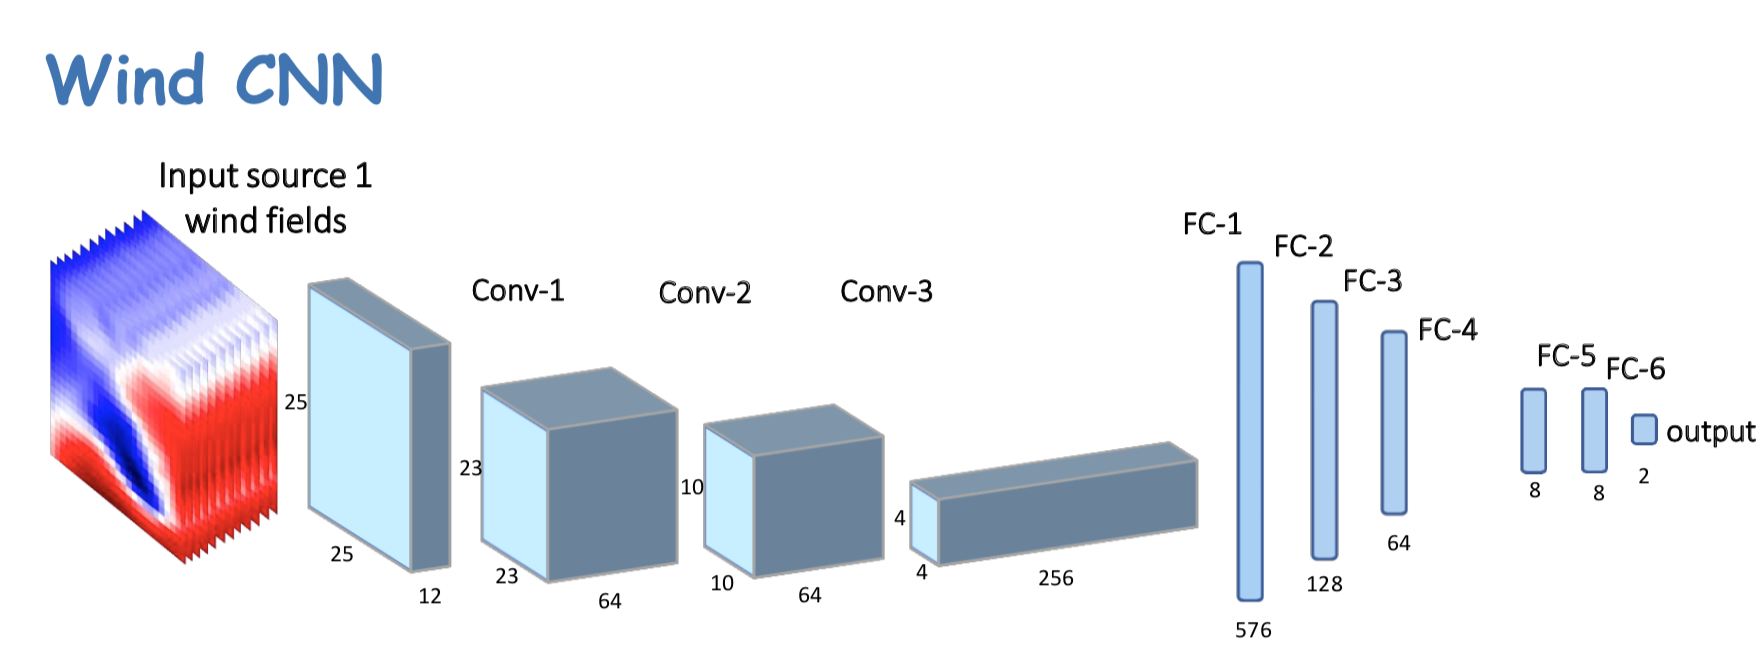
\includegraphics[width=0.8\linewidth]{figs/wind-cnn.png}
\end{figure}
\end{frame}

\begin{frame}
\frametitle{Train Stream Networks}
\begin{itemize}
	\item  Stage \Rmnum{1}: Train stream networks \\
	\begin{itemize}
		\item Pressure CNN
		\begin{itemize}
			\item same principle...
		\end{itemize}
		\item Past tracks + meta NN
			\begin{itemize}
				\item a simple multi-layer perception (MLP)
			\end{itemize}
	\end{itemize}
\end{itemize}
\begin{figure}

	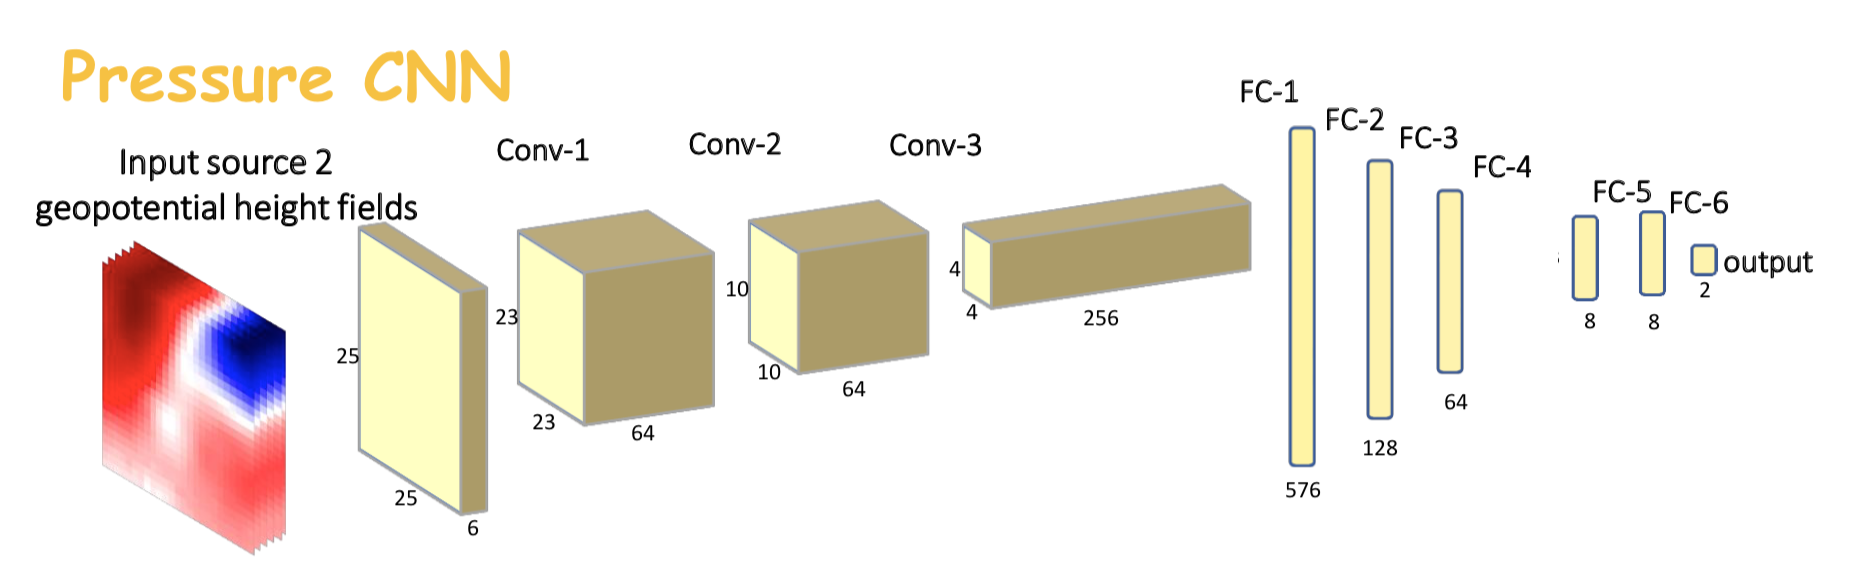
\includegraphics[width=0.65\linewidth]{figs/pressure-cnn.png} \\
	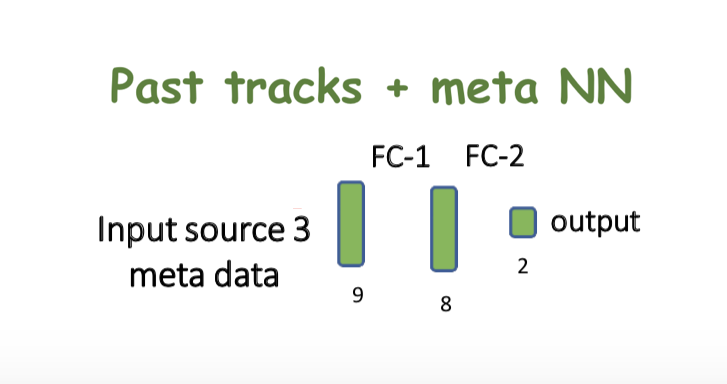
\includegraphics[width=0.32\linewidth]{figs/meta-nn.png}
\end{figure}
\end{frame}



\begin{frame}
\frametitle{Train Fusion Network}
\begin{itemize}
	\item  Stage \Rmnum{2}: Train the fusion network \\
\end{itemize}
\begin{figure}
	
	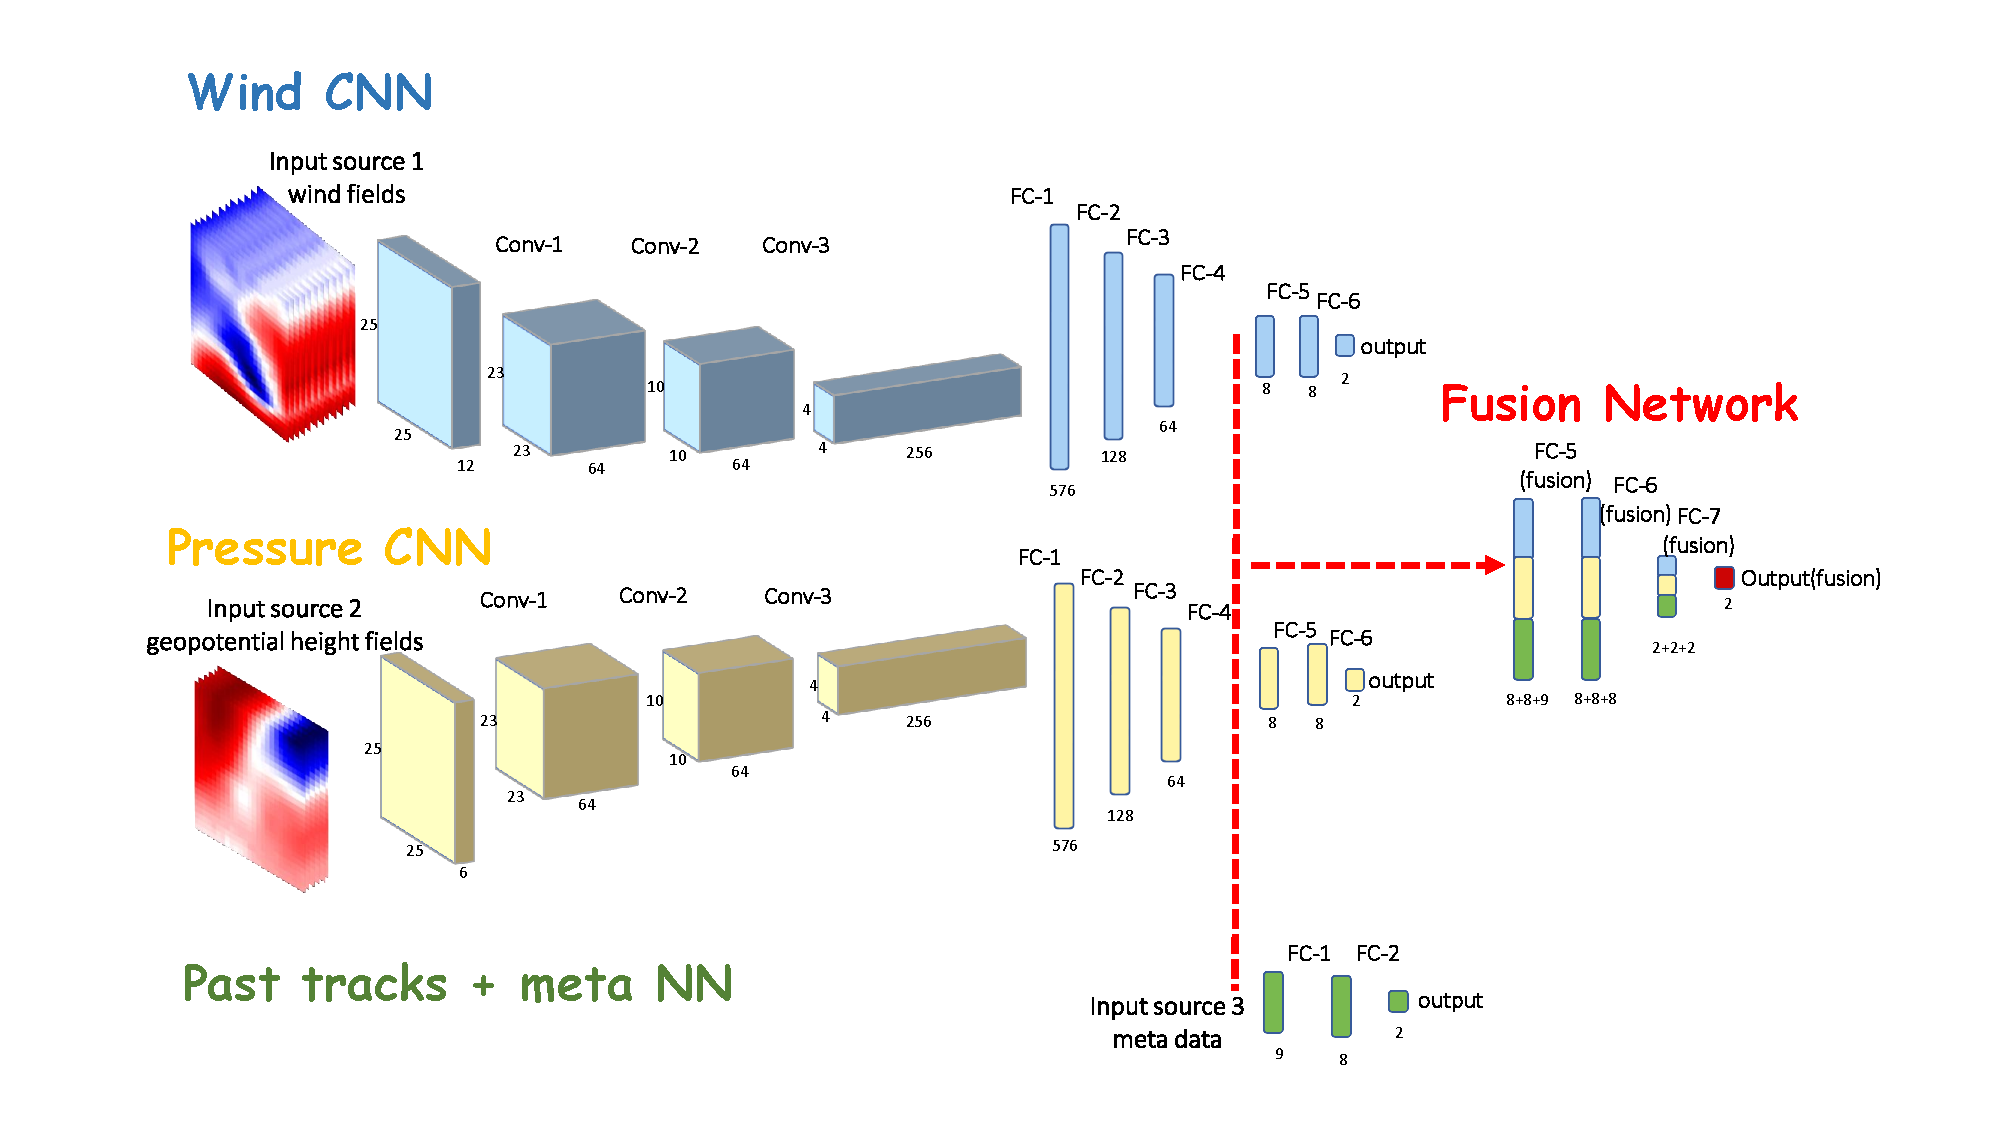
\includegraphics[width=0.8\linewidth]{figs/fusion_network.pdf} \\
	
\end{figure}
\end{frame}

\begin{frame}
\frametitle{Train Fusion Network}
\begin{itemize}
	\item  Stage \Rmnum{2}: Train the fusion network \\
	\begin{itemize}
		\item  zoom in fusion layers
		\begin{figure}
			\flushleft
			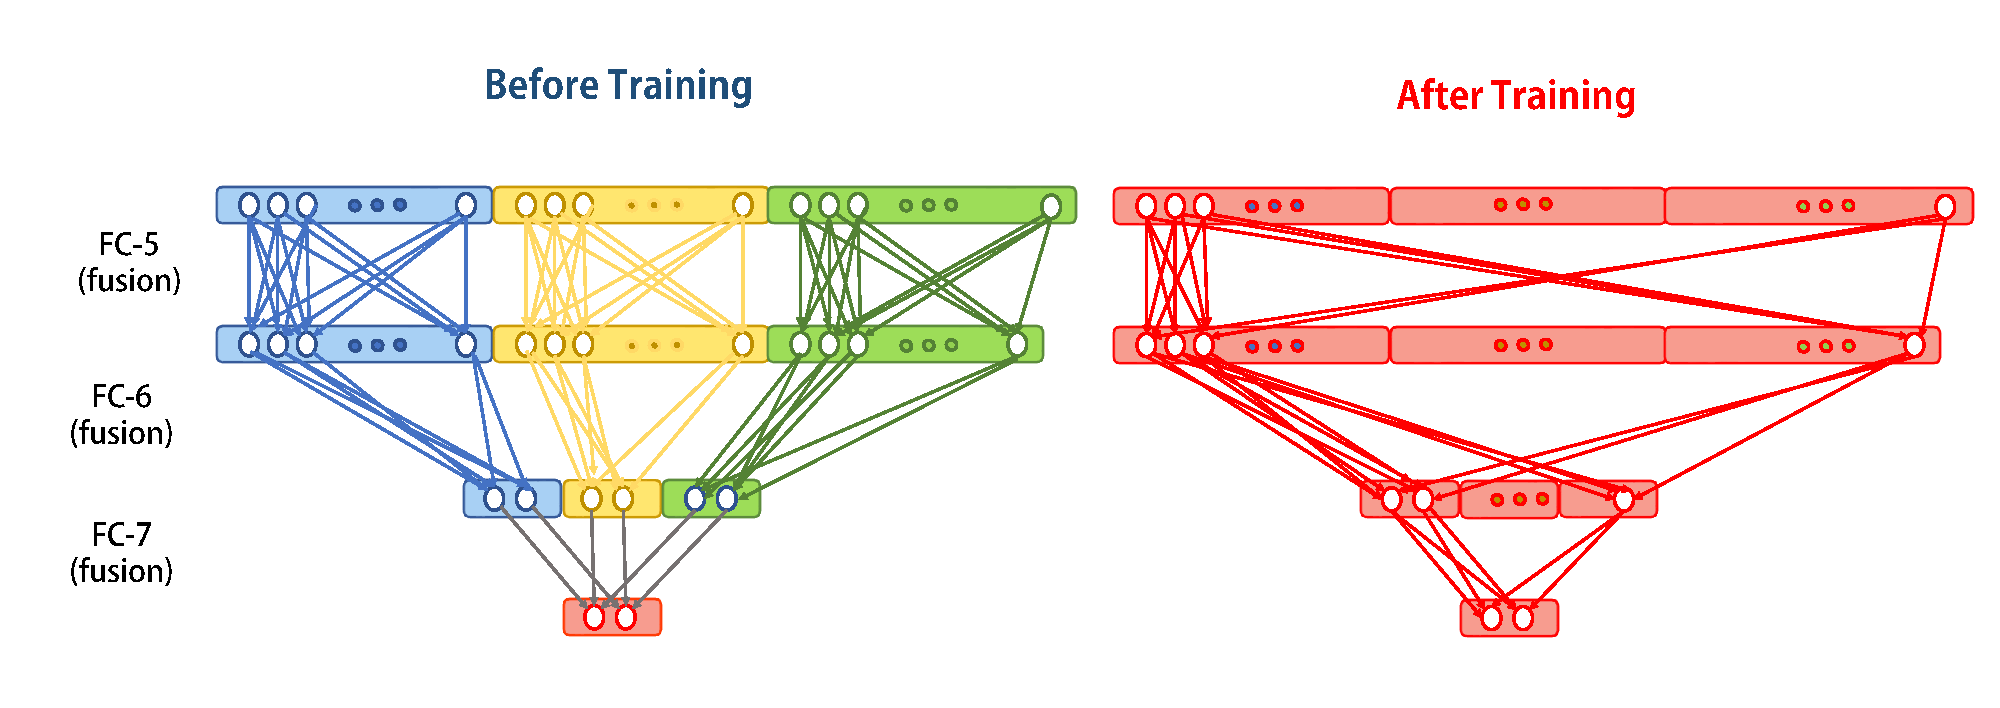
\includegraphics[width=0.65\linewidth]{figs/fusion_details.pdf} \\
		\end{figure}
		\item connections between different streams in fusion layers are added
		\item two-phase optimization:
			\begin{itemize}
				\item first phase: optimize weights only in fusion layers
				\item second phase: optimize weights in all layers
			\end{itemize}
	\end{itemize}
\end{itemize}
\end{frame}

\begin{frame}
\frametitle{Input preprocessing}
\begin{itemize}
	\item  the entire dataset into train (60\%) / validation (20\%) / test (20\%)
	\item separate all the storms into the three bins to avoid data leakage
	\item standardization
\end{itemize}
\end{frame}

\begin{frame}
\frametitle{Loss function}
\begin{itemize}
	\item Stage \Rmnum{1}: train independently three stream networks
	\begin{equation*}
	\label{eq}
	L(\theta_w) = \frac{1}{n}\sum_{i=1}^{n} \left \| {M_{transform}((F_{wind}(x_w^i; \theta_w)} + loc^i_{t} ) - loc^i_{t+\delta t} ) \right \| ^2
	\end{equation*}
	\begin{itemize}
		\item above showed Wind CNN loss function, analogical for other two stream networks.
		\item $\delta t$: the prediction interval
		\item $(x_w^n, x_p^n, x_{1d}^n, loc_t^n, loc_{t+\delta t}^n)\}$ : labeled data
		\item $\theta_{w}$: Wind CNN parameters
		\item $F_{wind}$: Wind CNN (input: wind fields $\mapsto$ output: expected displacement)
		\item $M_{transform}$: transformation matrix from differences in latitude and longitude to distance in kilometers
	\end{itemize}
\end{itemize}
\end{frame}


\begin{frame}
\frametitle{Loss function}
\begin{itemize}
	\item Stage \Rmnum{2}: train the fusion network (2 phases)
	\begin{equation*}
	\label{eq_fusion_2}
	L(\theta_{f}, \theta_{s}) = \frac{1}{n}\sum_{i=1}^{n} \left \| {M_{transform}((F_{f}(x_w^i, x_p^i, x_{1d}^i; \theta_{f}, \theta_{s})} + loc^i_{t} ) - loc^i_{t+\delta t} ) \right \| ^2
	\end{equation*}
	\begin{itemize}
		\item $\theta_{f}$: parameters of fusion layers 
		\item $\theta_{s}$: parameters of stream layers
		\item $F_{f}$: Fusion network (input: wind fields + pressure fields + 1d features (past tracks + meta) $\mapsto$ output: expected displacement)
	\end{itemize}
	\item first phase:  optimize only $\theta_{f}$
	
	
	\item second phase: optimize on $\theta_{f}$ and $\theta_{s}$

\end{itemize}
\end{frame}



\begin{frame}
\frametitle{Algorithmic Details}
\textbf{Algorithmic details:} ReLU, batch norm, adam, batch size=$256$, L2 $coeff.$ = $0.01$, fine-tuned initial learning rate, $He$ initialization \cite{he2015delving}... \textbf{No magic!}
\end{frame}








\section{Experiments}
\begin{frame}
\frametitle{Outline} % Table of contents slide, comment this block out to remove it
\tableofcontents[currentsection] % Throughout your presentation, if you choose to use \section{} and \subsection{} commands, these will automatically be printed on this slide as an overview of your presentation
\end{frame}

\begin{frame}
\frametitle{The Stream Networks}
\begin{figure}
	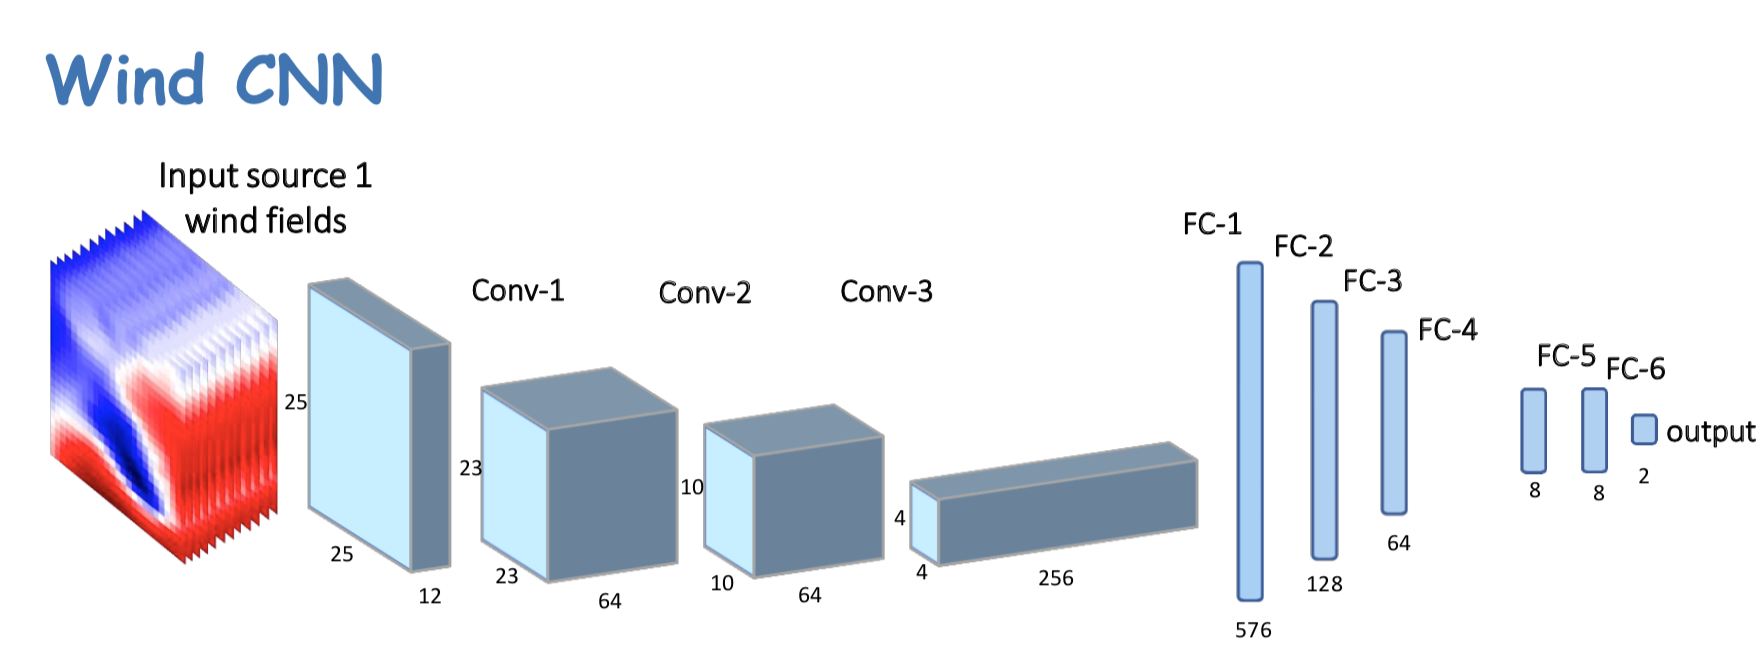
\includegraphics[width=0.8\linewidth]{figs/wind-cnn.png}
\end{figure}
\end{frame}

\subsection{Selecting Network Configurations}
\begin{frame}
\frametitle{Experiments}
\framesubtitle{Selecting Stream Network Configuration}
\begin{itemize}
	\item  Four candidates' network configurations for Wind CNN\\
	\begin{itemize}
		\item followed the same generic design
		\item from shallow to deep
	\end{itemize}
\end{itemize}
\begin{figure}
	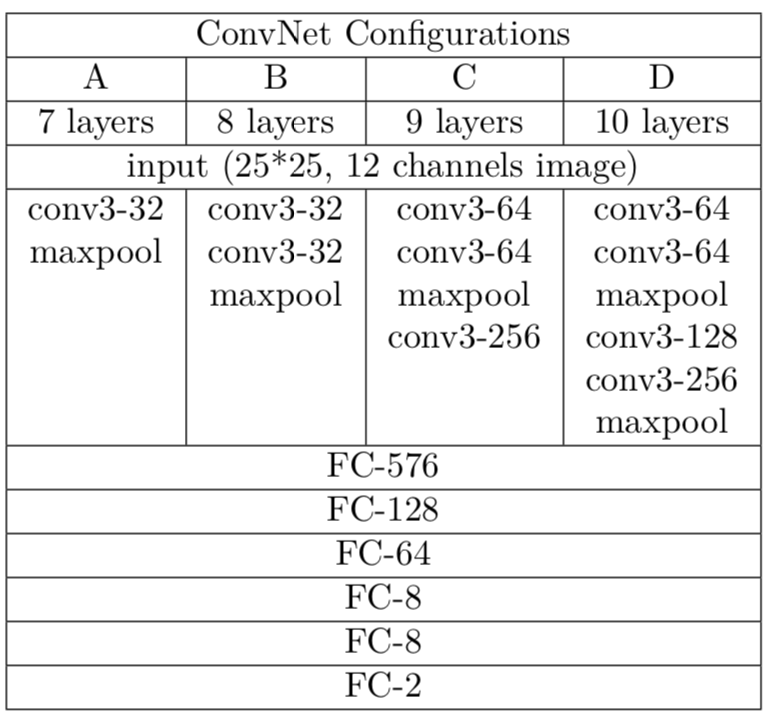
\includegraphics[width=0.4\linewidth, height=0.5\textheight]{figs/candidates.png} \\
\end{figure}
\end{frame}

\begin{frame}
\frametitle{Experiments}
\framesubtitle{Selecting Stream Network Configuration}
\begin{itemize}
	\item  Evaluation results on 24 hours of storm track prediction on the validation set (\textbf{A,B,C,D from shallow to deep})\\

\begin{table}[]
	\centering
	\begin{tabular}{|c|c|c|}
		\hline
		Model& Mean Square Error ($km^2$) & Mean Absolute Error($km$) \\ \hline
		A & 31430.08 & 145.43  \\ \hline
		B & 31761.95 & 146.62  \\ \hline
		C & 31552.91 & 145.5997 \\ \hline
		D & 31772.62 & 146.73 \\ \hline
	\end{tabular}
\end{table}
	\item Adding more temporal parts (storm fields data at the same location at more consecutive time steps to input data)
	\begin{itemize}
		\item  No noticeable improvement\\
	\end{itemize}
\end{itemize}
\end{frame}

\begin{frame}
\frametitle{Experiments}
\framesubtitle{Selecting Fusion Network Configuration}
\begin{itemize}
	\item  Three-stream fusion network \\
\end{itemize}
\begin{figure}
	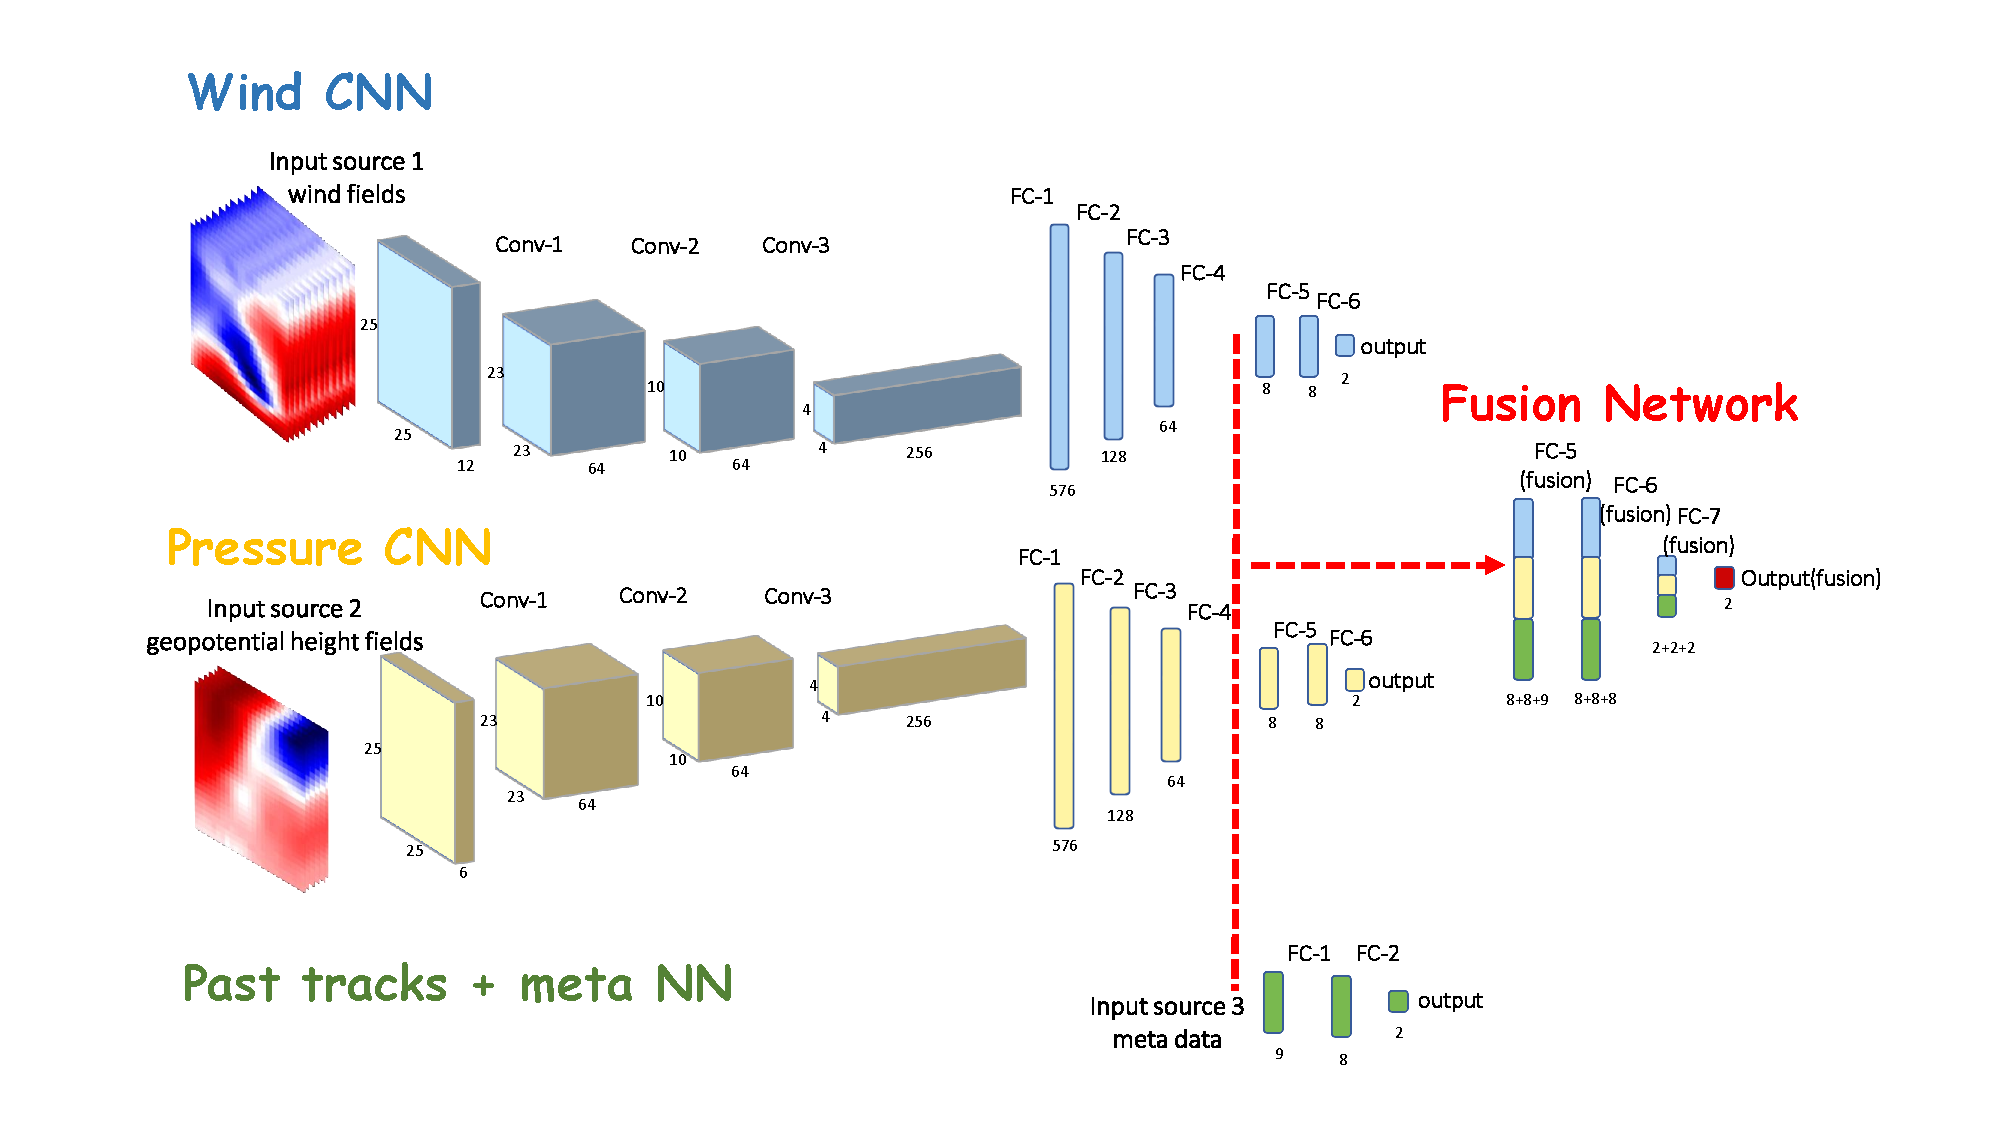
\includegraphics[width=1.0\linewidth]{figs/fusion_network.pdf}
\end{figure}
\end{frame}

\begin{frame}
\frametitle{Experiments}
\framesubtitle{Selecting Fusion Network Configuration}
Three scenarios:
\begin{itemize}
	\item  how many layers should be fused?
	\item  Does fusing three streams outperforms fusing two streams or using single stream?
	\item  Do we need to pretrain the 3 stream  networks before training the fusion networks?
\end{itemize}
\end{frame}

\begin{frame}
\frametitle{Experiments}
\framesubtitle{Selecting Fusion Network Configuration}
\begin{itemize}
	\item  how many layers should be fused?
	\begin{itemize}
		\item Comparison of fusion networks that fuse different number of layers on 24 hours storm track prediction on \textbf{validation set}.
		
	\end{itemize}
	\begin{figure}
		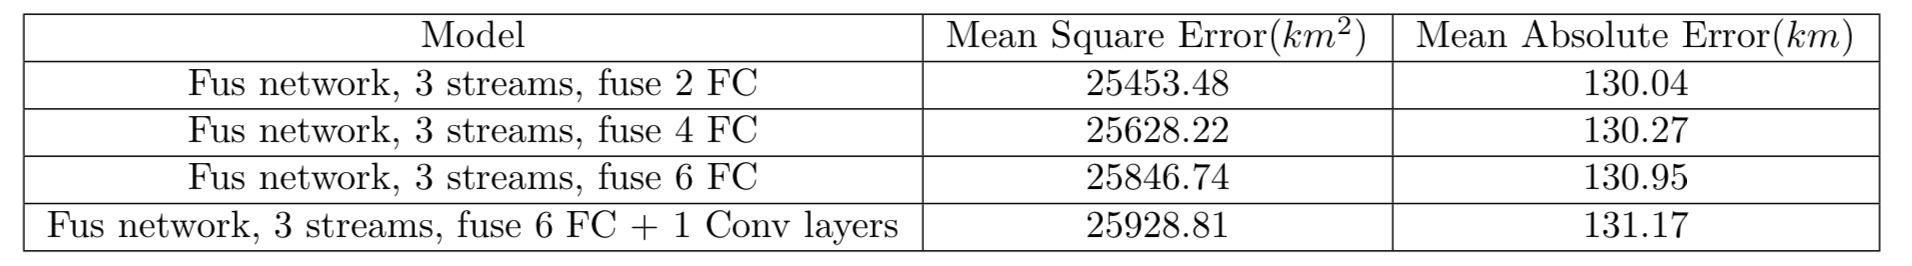
\includegraphics[width=0.95\linewidth]{figs/fusion_1.png} \\
	\end{figure}
	\item  Does fusing the three streams outperforms fusing two streams or using single stream?
	\begin{itemize}
		\item Comparison between the fusion network fusing all three streams with networks fusing two streams and single stream networks.
		\item compare also with naive fusion (no pretrain)
		\item Result shown in the next slide
		
	\end{itemize}
\end{itemize}
\end{frame}

\begin{frame}
\frametitle{Experiments}
\framesubtitle{Selecting Fusion Network Configuration}
\begin{figure}
	\caption{24h-forecast results, in distance between predicted and real location.}
	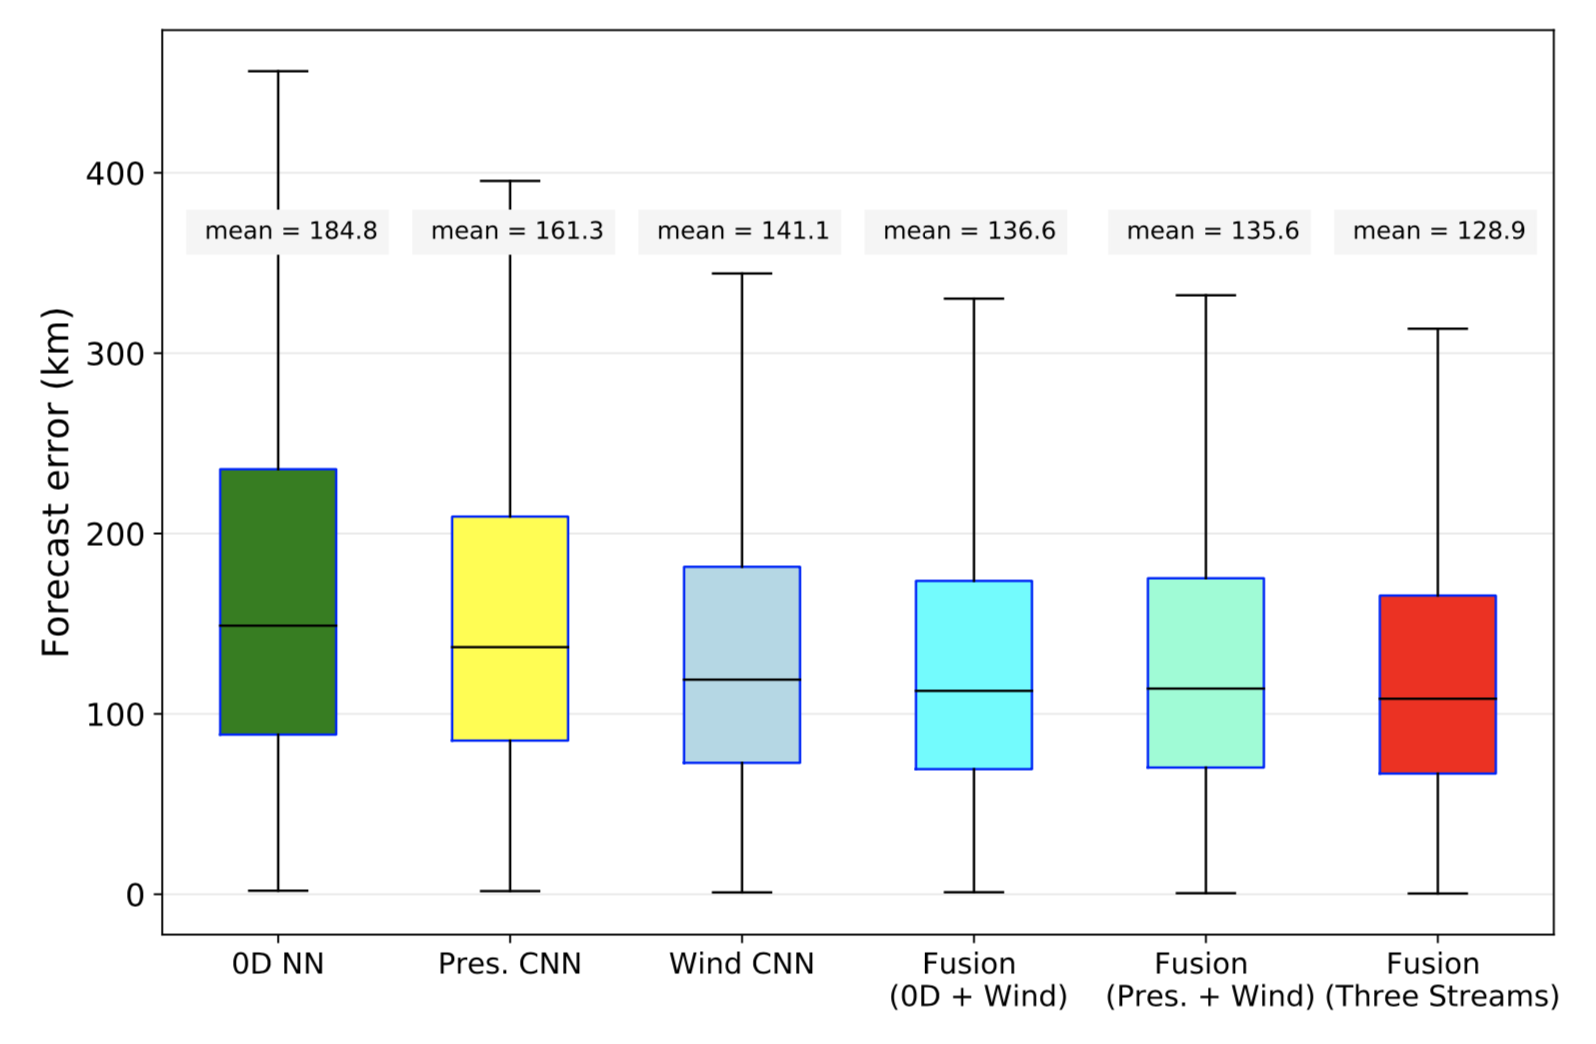
\includegraphics[width=0.68\linewidth]{figs/MAE.PNG} \\
\end{figure}

\small{naive fusion's forecasting error in distance: \textbf{142.63 km}, worse than best single stream alone! }


\end{frame}


\subsection{Comparison with the Existing Forecasting Models}
\begin{frame}
\frametitle{Outline} % Table of contents slide, comment this block out to remove it
\tableofcontents[currentsubsection] % Throughout your presentation, if you choose to use \section{} and \subsection{} commands, these will automatically be printed on this slide as an overview of your presentation
\end{frame}

\begin{frame}
\frametitle{Experiment} 
\framesubtitle{Comparison with the Existing Forecasting Models}
\begin{itemize}
	\item Compare with: A standard statistical model (BCD5)
	\item Also compare with: Official NHC forecast (OCFL).Ensemble methods, imporved over years
	
\end{itemize}
\end{frame}


\begin{frame}
\frametitle{Experiments}
\framesubtitle{Comparison with the Existing Forecasting Models}
Quantitative: 
\begin{figure}
	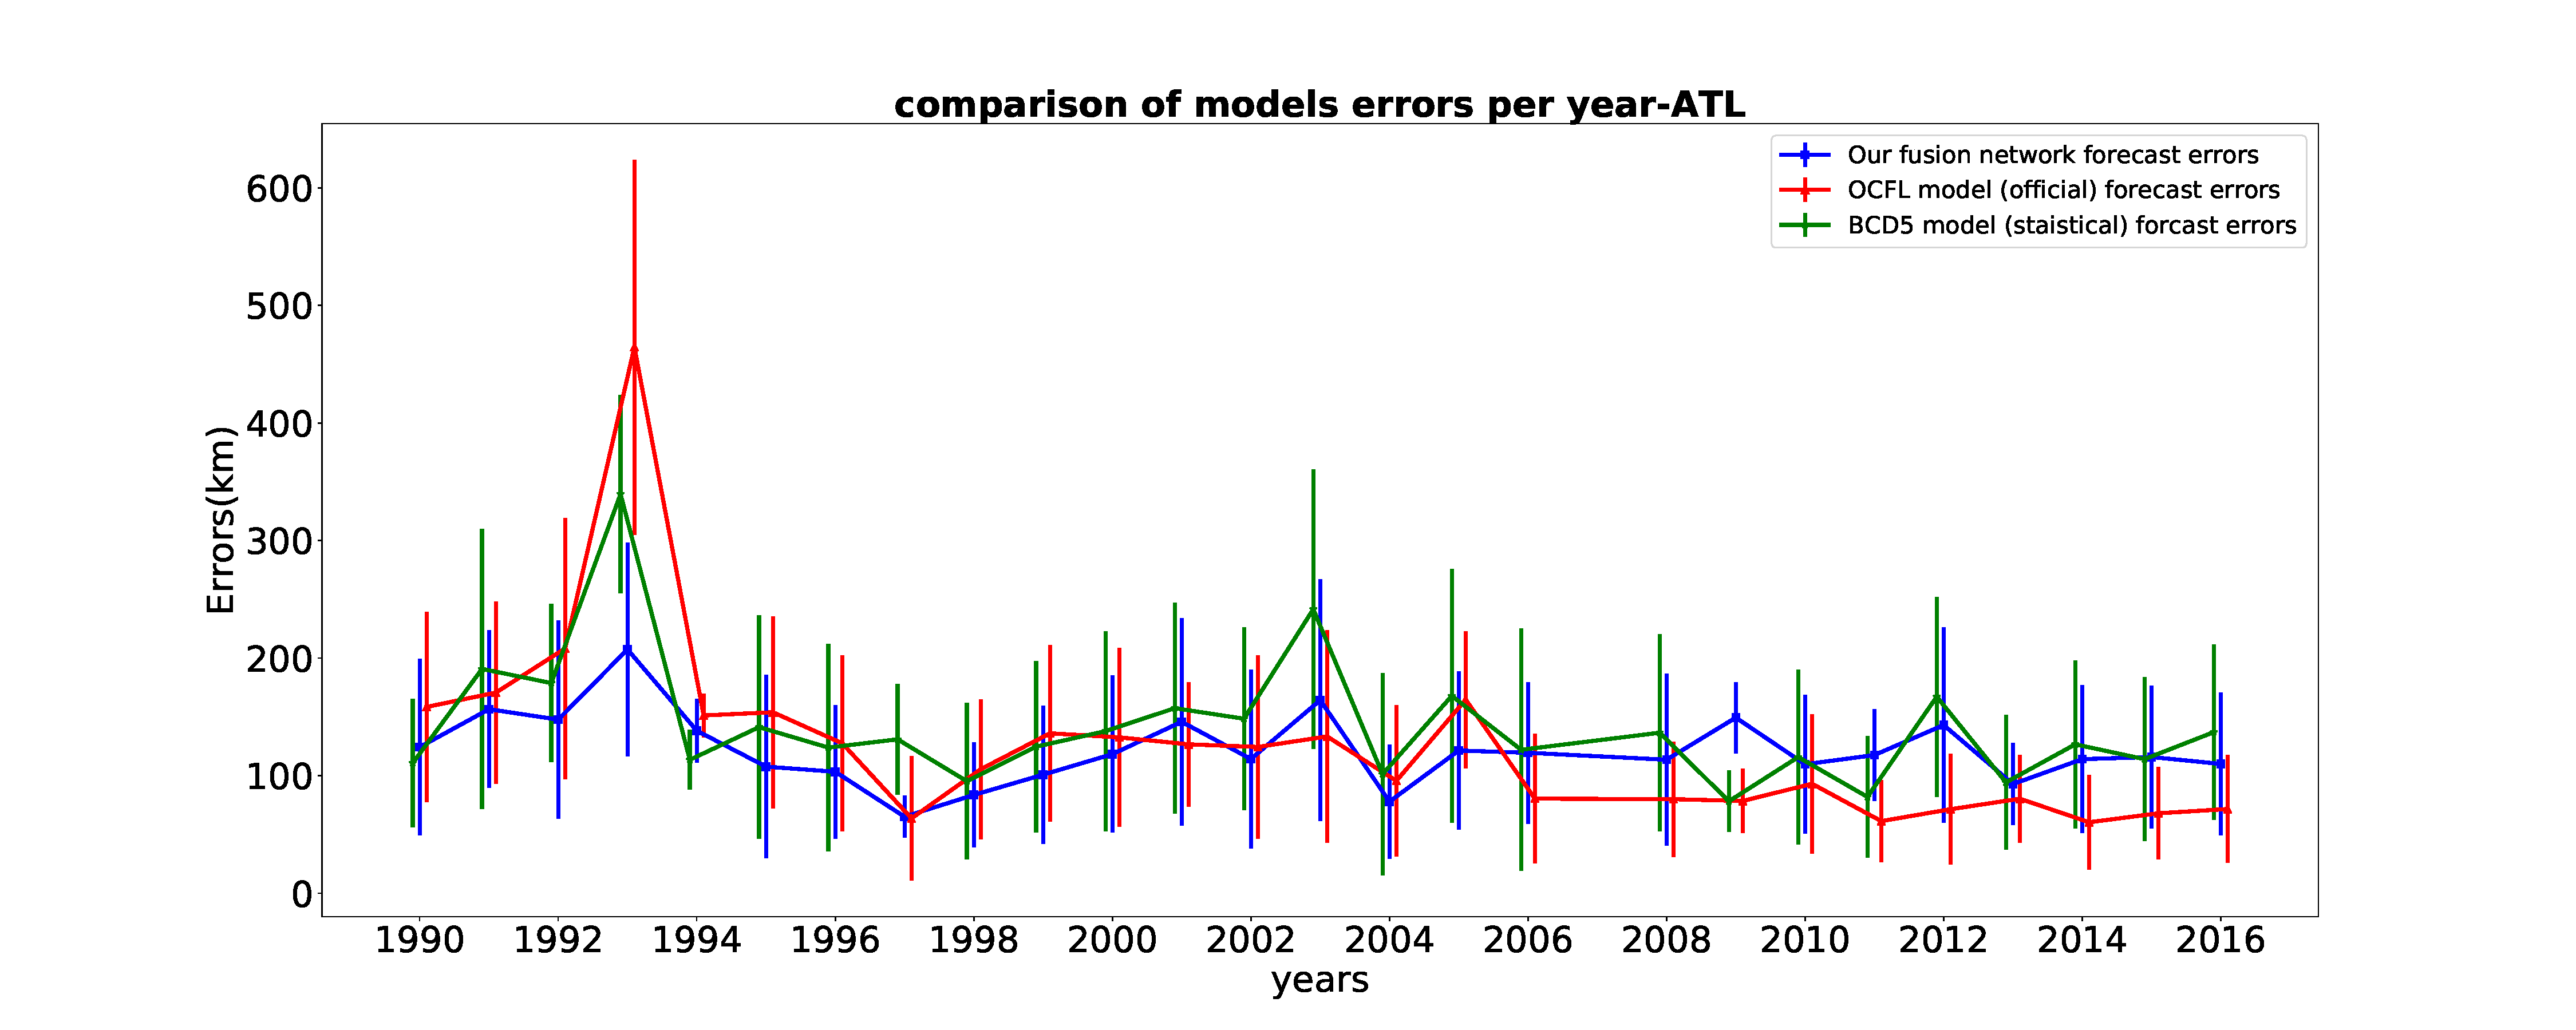
\includegraphics[width=1.0\linewidth]{figs/ATL_comparison_of_models_errors_per_year.pdf}\\
	\caption{The yearly average 24-hours storm track forecasting errors (km) and standard deviation on the test set in \textbf{Atlantic} for our fusion network forecasts(blue), the BCD5 (green) and the OFCL (red), 1989-2016.}
\end{figure}
\end{frame}

\begin{frame}
\frametitle{Experiments}
\framesubtitle{Comparison with the Existing Forecasting Models}
Quantitative: 
\begin{figure}
	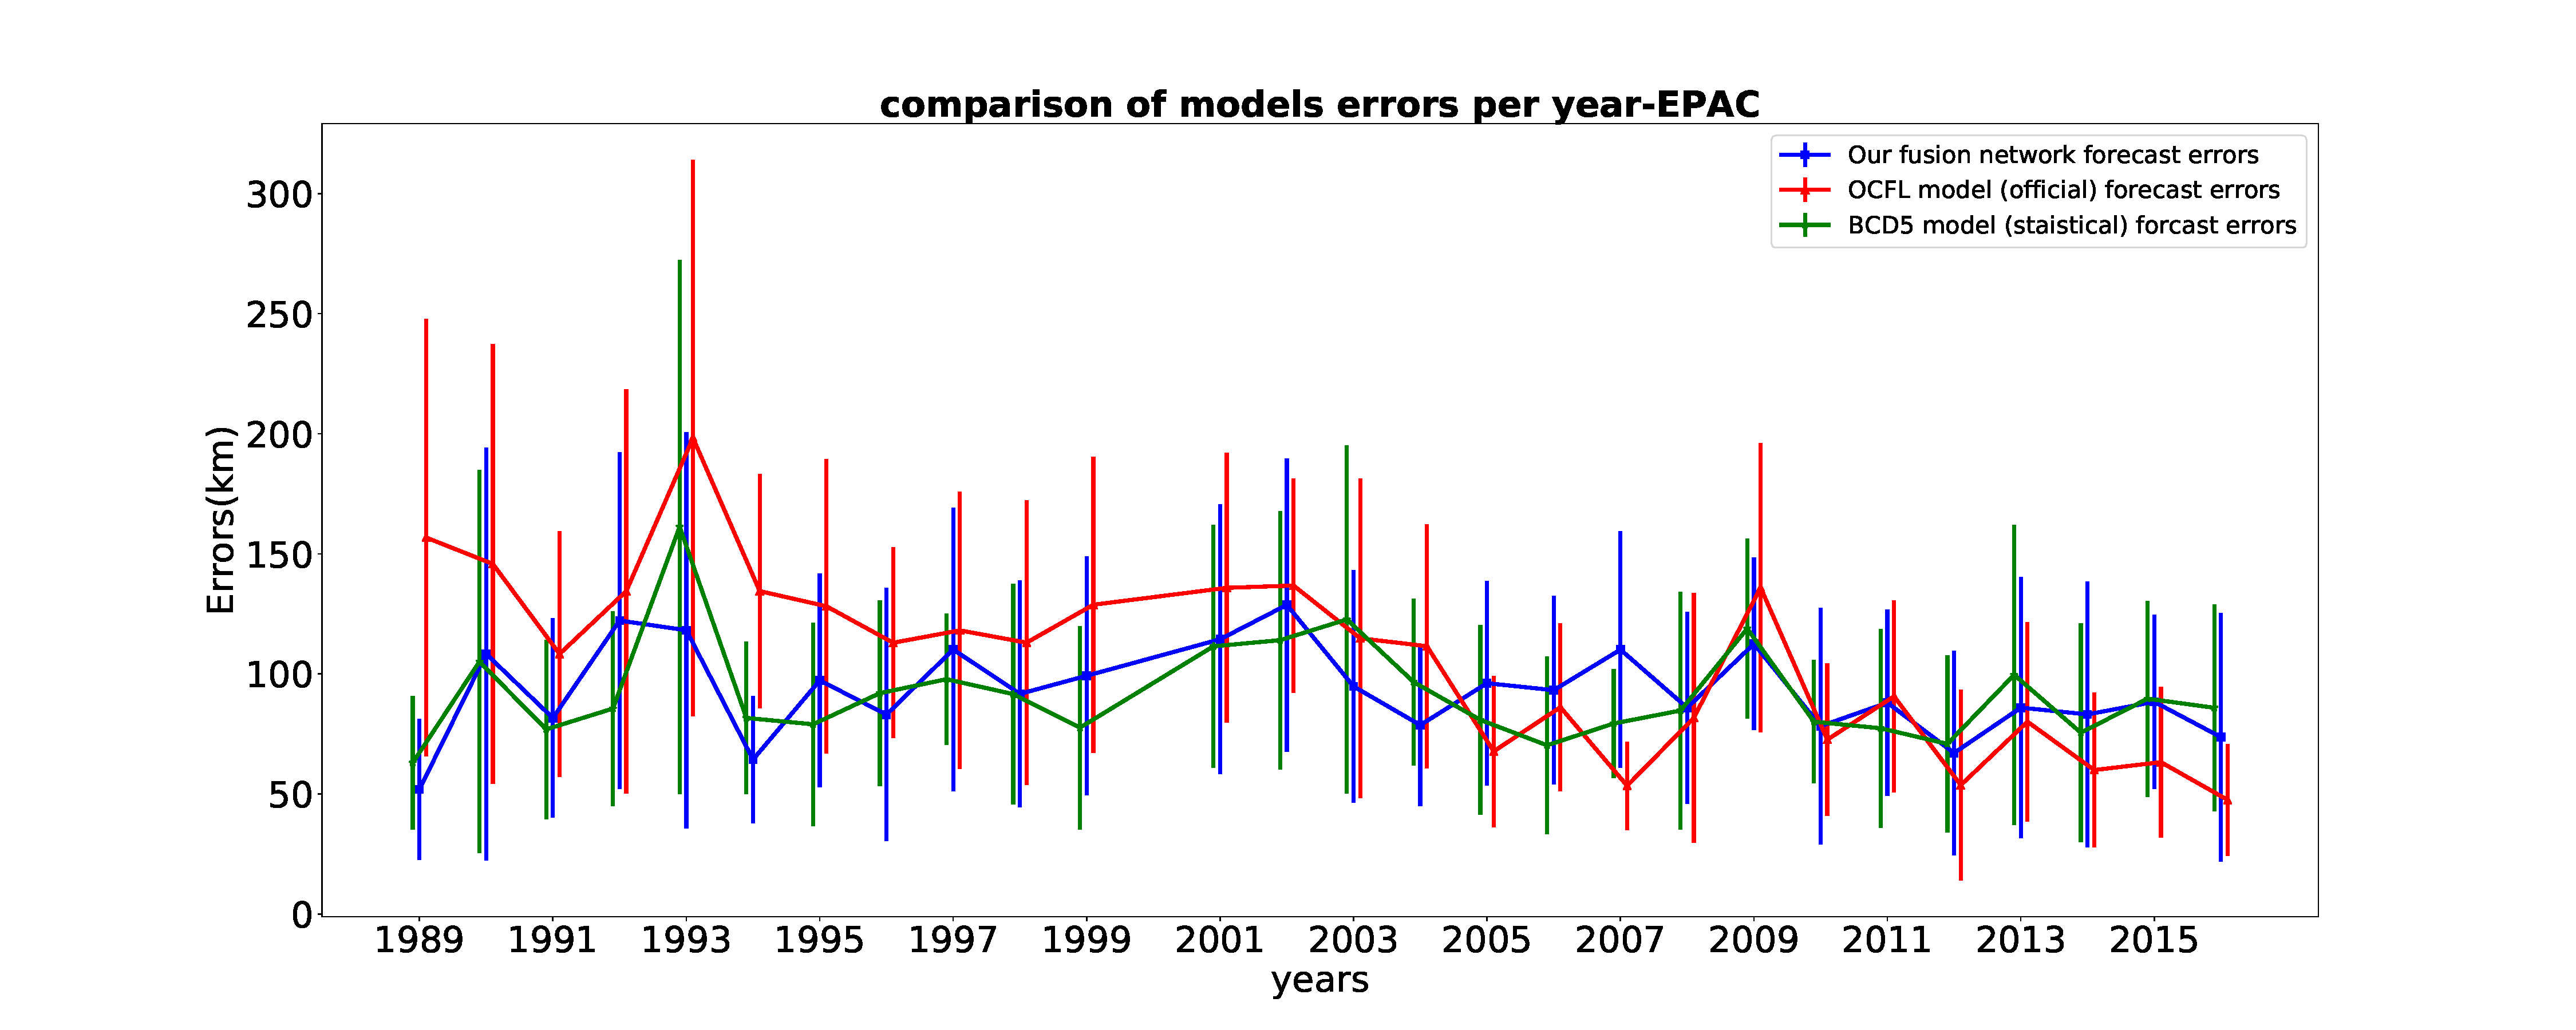
\includegraphics[width=1.0\linewidth]{figs/EPAC_comparison_of_models_errors_per_year.pdf}\\
	\caption{The yearly average 24-hours storm track forecasting errors (km) and standard deviation on the test set in \textbf{East Pacific} for our fusion network forecasts (blue), the BCD5 (green) and the OFCL (red), 1989-2016.}
\end{figure}
\end{frame}

\begin{frame}
\frametitle{Experiments}
\framesubtitle{Comparison with the Existing Forecasting Models}
Quantitative: \\
\begin{itemize}
	\item Mean storm track forecast errors of all years in the two basins (Atlantic and Pacific) on the test set for our fusion network and BCD5 model: 
\end{itemize}

\begin{figure}
	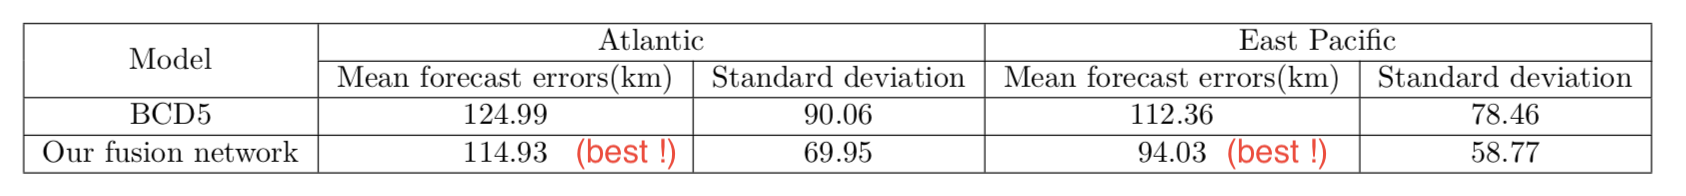
\includegraphics[width=1.0\linewidth]{figs/compare_with_baseline}\\
\end{figure}
\end{frame}

\begin{frame}
\frametitle{Experiments}
\framesubtitle{Comparison with the Existing Forecasting Models}
Qualitative: 

\begin{figure}
	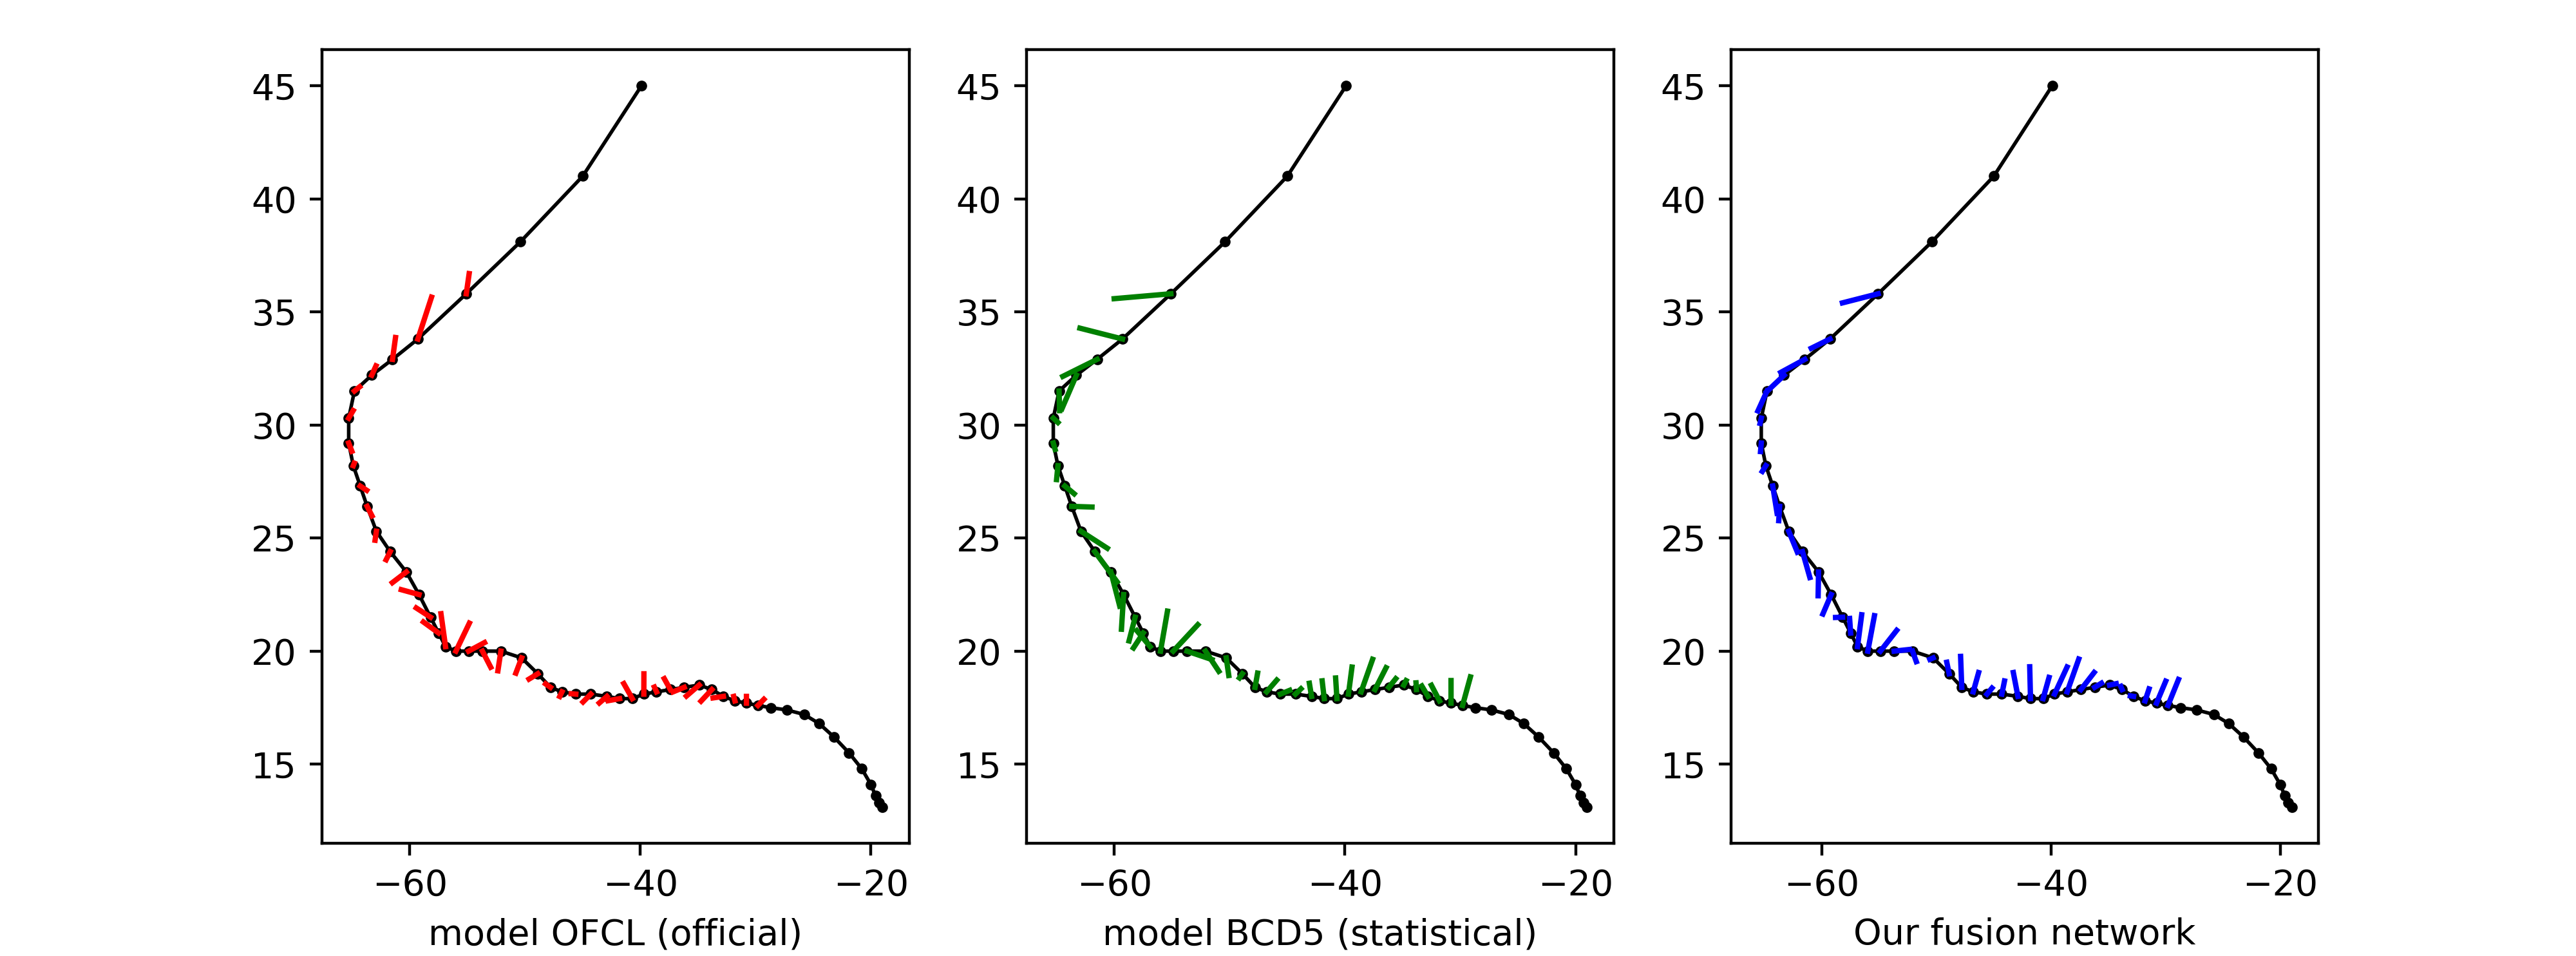
\includegraphics[width=1.0\linewidth]{figs/one_stom_result.png}\\
	\caption{The forecast errors of the three models (left: the OCFL, middle: the BCD5, right: our fusion network) on the Hurricane Ian in 2016}
\end{figure}
\end{frame}

\begin{frame}
\frametitle{Experiments}
\framesubtitle{Comparison with the Existing Forecasting Models}
Qualitative: 

\begin{figure}
	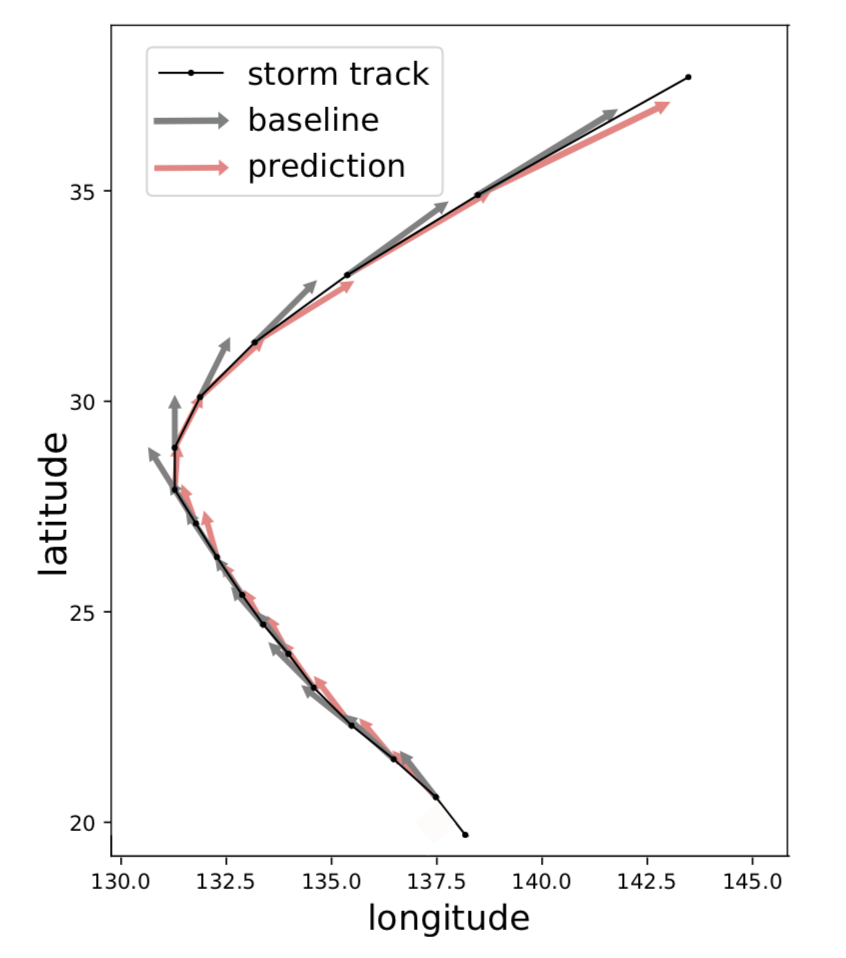
\includegraphics[height=0.6\textheight, width=0.4\linewidth]{figs/6h_track.png}\\
	\caption{\small{Example of 6h-forecasts on one storm track. The baseline prediction is equal to the last 6h-displacement (going straight).}}
\end{figure}
\end{frame}

\section{Discussion}
\begin{frame}
\frametitle{Discussion}
\large{Conclusion:}

\begin{itemize}
	\item  Proposed a promising deep learning framework for storm track forecasting
	\item  Designed a fusion network consists of a three-stream convolutional neural network that can learn to fuse information from both atmopheric fields and history track
	\item  our model outperforms the BCD5 model
	\item  our model can help to enhance the official forecast, even its forecast errors are larger than the OFCL model.
\end{itemize} 
\end{frame}

\begin{frame}
\frametitle{Discussion}
\large{What's next?}

\begin{itemize}
	\item  Design an algorithm that could effectively learn information from high-dimensional tensor data.
	\item  Try unsupervised learning algorithms (e.g. clustering)
	\item  Apply multi-target learning
\end{itemize} 
\end{frame}

\begin{frame}
\Huge{\centerline{THANK YOU}}
\small
\begin{itemize}
	\item work published in Climate Informatics Workshop Proceedings 2018, Sep 2018, Boulder, United States: 'Fused Deep Learning For Hurricane Track Forecast From Reanalysis Data' (same title)
	\item \textbf{advertisement:} Data challenge (Hackson) of Saclay Datascience Center about hurricane intensity forecast is going to be hold in Boulder, United States, Oct.
\end{itemize}
\end{frame}


\bibliographystyle{apalike}   
\bibliography{presentation.bib}
\end{document}